\documentclass[11pt]{article}
\usepackage{amsmath,amssymb,amsthm,mathtools}
\usepackage{graphicx, listings, siunitx}
\usepackage[margin=1in]{geometry}
\usepackage{fancyhdr}
\setlength{\parindent}{0pt}
\setlength{\parskip}{5pt plus 1pt}
\setlength{\headheight}{13.6pt}
\newcommand\header[1]{\vspace{.25in}\hrule\textbf{#1}\vspace{.5em}\hrule\vspace{.10in}}
\renewcommand\part[1]{\vspace{.10in}\textbf{(#1)}}
\DeclarePairedDelimiter\ceil{\lceil}{\rceil}
\DeclarePairedDelimiter\floor{\lfloor}{\rfloor}
\pagestyle{fancyplain}
\lhead{EE16B Spring 2016}
\rhead{Project SIXT33N GSI Readme | \PHASE}


\lstset{
    frame=single,
    breaklines=true,
}

\begin{document}\raggedright
\newcommand\NAME{Emily Naviasky}  % your name
\newcommand\PHASE{Phase 1: Circuits}

\LARGE \textbf{Project SIXT33N GSI Readme}

\Large \textbf{\PHASE}
\normalsize

Dear 16B Lab TA,

Here is what we think you would like to know about this phase. We suggest you read this with the iPython Notebook for this section open. 

Good Luck.

Sincerely,
Emily and Nathan

\header{Schedule}
Groups should be finished with schematic design by the first week so that they have the entire second week to build and debug their circuit. The second week will be a little tight if groups run into a bad bug, so make sure that students are getting debug help if they need it. They NEED to be finished with this circuit by the end of the second week because they will be using it in the third week. 

For this phase, the notebook tells students to check with the GSI very frequently. The purpose of this is that (for this phase in particular) if students run off in a bad direction too early it will waste a lot of time. You should have a pretty good idea of where each group is because of these frequent check ins and you should be able to keep them on track and help groups that are in trouble.


\header{Materials}
In this phase, students will need a couple special components in the cabinet. Each group should get EXACTLY 1 electret microphone and 1 potentiometer (we do not have spares). NO OTHER COMPONENT SHOULD BE DISTRIBUTED. Students are to use the components in the component bin and their own op-amps. If they need extra op-amps, tell them to get samples from TI online.

\header{Part 1}
In this part, students are just building the very first block of their microphone circuit. They check that their microphone works and get an idea of what the signal looks like without gain or filtering. 

They are meant to see evidence that a capacitor removes DC, and then they use the potentiometer to introduce a bias that is convenient. It is important that they are thinking about DC bias before they hit the next stage where they will have to think a lot about it.

Finally, students are told to note down the DC bias and peak to peak voltage. This is so that they can use them in their block and schemtic designing. Make sure that they take those into consideration later to keep the final DC bias at 1.6V and have a output swing of 3.3V.

\textbf{Debugging:} There should not be much to get stuck on in this stage. 
\begin{itemize}
    \item Make sure that they have soldered leads onto their mic, because the mic leads don't always make contact with the breadboard.
    \item When students are looking at their scope output, make sure that their volts/div is zoomed in reasonably far and that their time scale is in the ms range.
    \item If students don't see a signal, make sure mic is not backwards.
    \item The positive terminal of the mic should be at around 2V. If it is 5V or 0V, check the microphone polarity. If it is inserted correctly, there is a large chance they burnt the microphone when soldering wires to the leads.
    \item If the potentiometer is not enough to adjust the output level to 1.6V, add resistors in series with the bottom resistor or the top resistor in the divider. This is likely due to the matching of the $1M\Omega$ resistors.
\end{itemize}


\header{Part 2}
The trickiest part of this design is how students choose to deal with the DC bias. The next trickiest is implementing the second order filter. Everything else they should have dealt with in the FE lab.

The first thing that students will come to you with is their block diagram. This is the first place to check and make sure that students have some plan to deal with the DC bias. If they do not have some mention of level shifting or bias voltage, use their own diagram to walk them through what will happen when a DC signal goes through a gain stage. Next, make sure that they have either a second order filter, a first order active filter followed by a passive filter, or two passive filters with a buffer in between.

The schematic is where you will see how they deal with these problems in particular once you are sure that they recognize what all of the problems and specs are. It is likely that you will have to explain some theory around ground and DC biasing here. The best students might understand that they need define their own virtual "ground". Most students will have to be walked through the thought process of how to remove a bias. Make sure you have a good explanation handy. 

Usually, it works pretty well to get them to think of "defining a new ground". In the FE lab circuit, the circuit has -5V and 5V supplies, so the signal can be centered at 0V. This center is their reference, which is their "ground". In this circuit, their output is between 0V and 3.3V, so their signal needs to be centered at 1.65V. This should their "reference", or "ground". You can also think of this as shifting the whole circuit up by 1.65V by replacing all nodes that were ground by some 1.65V node. They can create the 1.65V reference with a voltage divider and a buffer. 

\textbf{NOTE:} If students want to build a Sallen-Key filter, Make sure the gain of the filter is 1 (i.e. have a buffer instead of a gain stage). If the gain is larger than 1, the filter might oscillate and students would create a clock instead of a filter. In theory a gain could be achieved but the R and C values need to be carefully chosen, but avoid this to make your life easier.

\textbf{The TA solution}: 
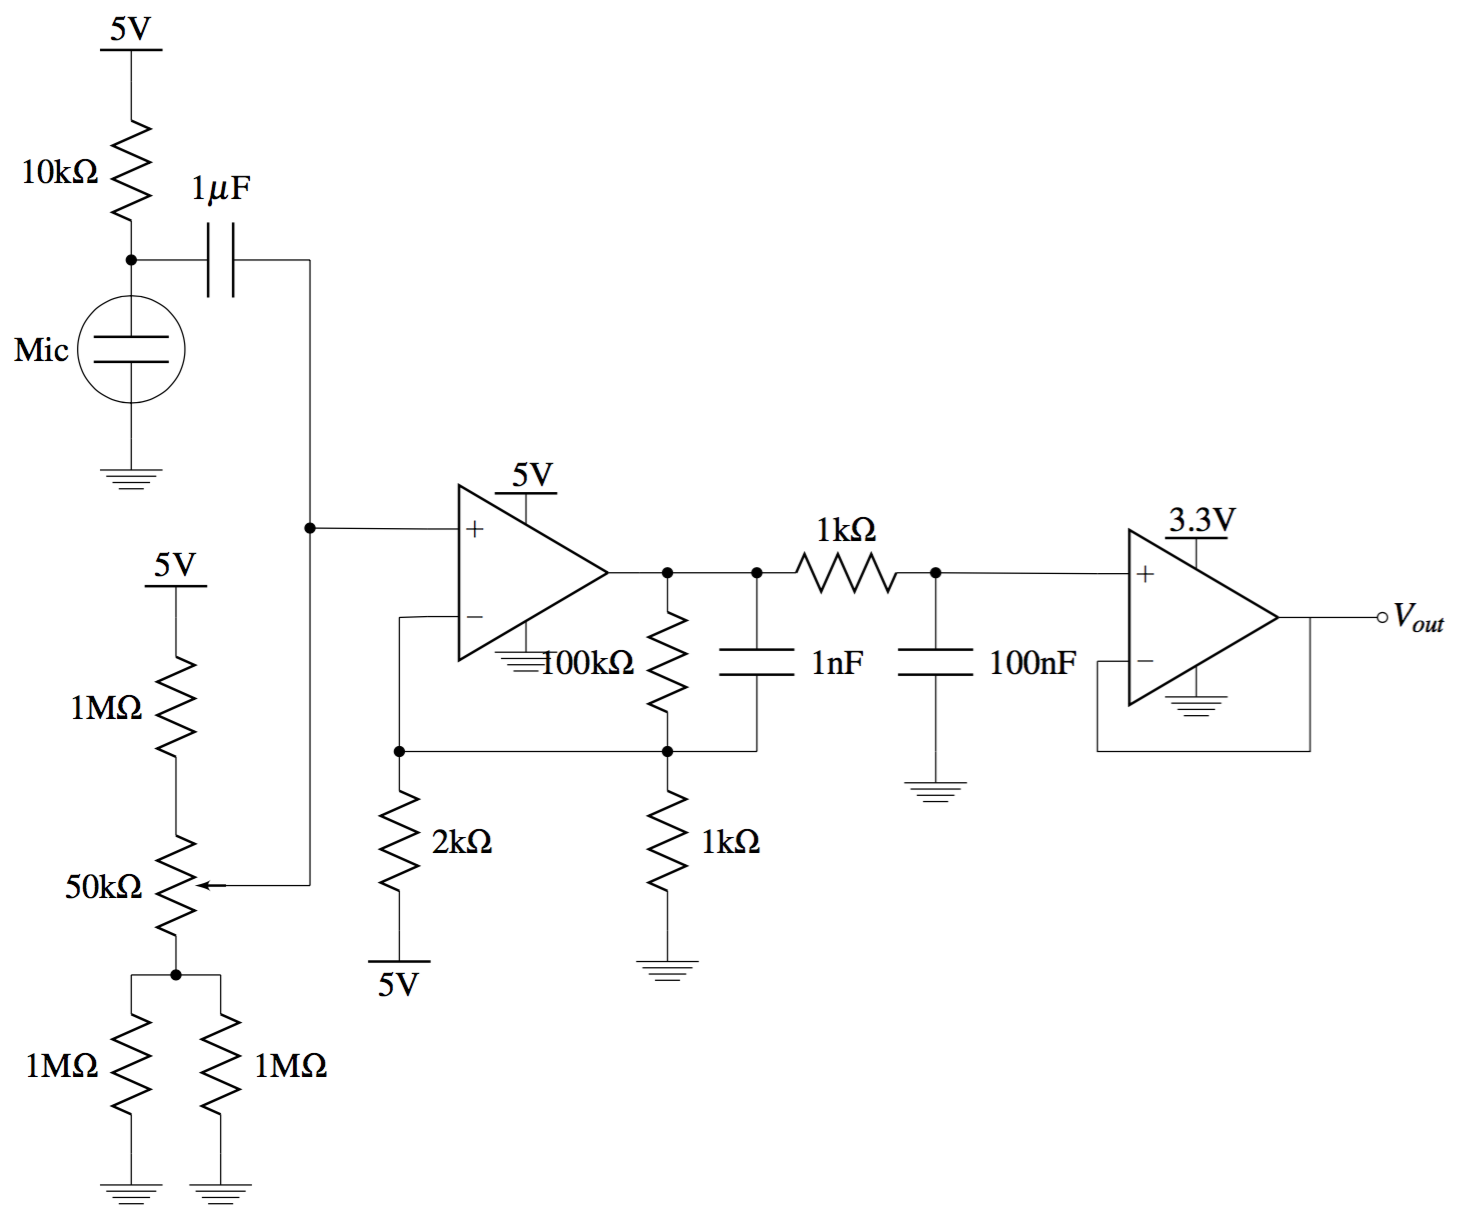
\includegraphics[width=\linewidth]{../proj-fe.png}
This circuit has a non-inverting active low-pass filter cascaded with a first-order passive filter. The amplifier plays a similar game by putting the reference "ground" at 1.6V, but incorporating the voltage divider into the inverting amp instead of buffering it. At DC, the inverting input is at 1.6V while at signal frequency the resistors to ground and 5V act as parallel resistors which provides gain with the $100k\Omega$ in feedback. The passive low-pass filter does not need to go to 1.6V because we have a capacitor (and the DC level does not affect the behavior).

Note that the virtual ground does not have to be exactly at 1.65V. We have a potentiometer in the input that we can tune to counter small DC offsets.

Generally students would not come up with this solution, and you should not point them to this solution because it will be easier for them to debug their own circuit if they understand fully how it should behave.

\textbf{Debugging:} 
\begin{itemize}
    \item Check that students design for decent gain. The solution has a gain of 150 - in general, it should be between 100 and 200. To measure the signal amplitude, set the oscilloscope to take an average of 2 samples. This will eliminate noise and display only the signal. To do this, press the Acquire button in the oscilloscope. They should see their signal in the order of 20mV. If it is much smaller, make sure the microphone polarity is right.
    \item Once students start building, they might be tempted to probe both the mic output ($V_{mic}$) and somewhere else on the circuit to compare them. This is a bad idea, for a subtle reason. The scope probe has a lot of parasitic cap and the electret mic is very sensitive to this. Probing that node and trying to look at an output later in the circuit will mess up the careful biasing of their first stage and will cause the opamp to rail. Basically, once they have a first opamp stage, don't touch the $V_{mic}$ node any more.

    \item If gain seems low, check that students put their filter corner in the right place.
\end{itemize}

\header{Part 3}
This section is pretty straight forward and is just to make sure that students can collect good data. Some struggling students will not have noticed that their gain is too small until this point when they see the signal on the screen and it is too low.

\textbf{Debugging:} 
\begin{itemize}
    \item If the adc\_read python script is stalled, make sure that student programmed their launchpad with adc\_read.ino code.
    \item If the scope shows that the signal is strangely clipped or held low or high, make sure that student programmed their launchpad with adc\_read.ino code.
\end{itemize}

\end{document}
